\section{The ACIADDRI Model}
\label{sect:aciaddri}

This work is  based on flocking behavior that was proposed by Craig W. Reynolds
in 1987 and extends it by adding the support to coexistence and interaction
between different species and predator avoidance.
Reynolds was amongst the first to abstract this behaviour to steer a swarm
of simulated birds which he called boids\cite{Reynolds}(contraction of birdoid).
Every boid has some limitations:
it has a strictly local knowledge of the space it occupies and its knowledge
comes from a simulated vision from its current position, in other words there is
no centralized control. The flock takes its decisions in a totally distributed
manner in order to obtaining a synchronized movement. More specifically, he
considered three behavioural rules each bird obeys:

\begin{description}
\item[\textsc{Cohesion}] \hfill\\
	to attempt to stay close to nearby flockmates
\item[\textsc{Collision Avoidance/Separation}] \hfill\\
	to evade obstacles and flock mates which are too
close
\item[\textsc{Velocity/Heading matching}] \hfill\\
	also called \textit{alignment}, to move in the same direction as nearby flock
	mates.
\end{description}

The \textsc{Aciaddri} model describes the environment and each bird's specie  by
means of  sets of parameters as follows:


\subsection{Environment Parameter}
 The environment is described by means of its width, length, height and by the
 time step parameter i.e. the duration in seconds of a single computational
 step. 
 \begin{table}[h!]
	\centering
	\begin{tabular}{l l l l}
	\hline
	Name & Symbol & Dimension & Description\\
	\hline
	Length &  \(W_x\) & $\dimensional{L}$ & Length of the environment \\
	Height & \(W_y\) & $\dimensional{L}$ & Height of the environment \\
	Width & \(W_z\) & $\dimensional{L}$ & Width of the environment \\
	Time Step & \(t\) & $\dimensional{T}$ & computational step duration \\
	\hline
	\end{tabular}
	\caption[List of Environment Parameters]{List of Environment Parameters of Birds Flocking}
	\label{tab:EnvironmentParameters}
\end{table}


\(W_x\), \(W_y\), and \(W_z\) are the dimension of the environment that represent 1 pixel as 1 meter. \(t\) is computational duration where 1 time step equivalent to 1 processing time.

\subsection{Species Parameters}
Each specie is described by a set of parameter that represent quantities that
are involved in the flight and flocking dynamics.

\begin{table*}
\centering
	\begin{tabular}{|l | l| l| l|}
	\hline
	Name & Symbol & Dimension & Description\\
	\hline
	Size & $s$ & $\dimensional{L}$ & Size of the bird \\
	Peak Velocity & \(v_p\)  & $\dimensional{L}\dimensional{T^{-1}}$  & The maximum velocity\\
	Thrust 	& \(a\) & $\dimensional{L}\dimensional{T^{-2}}$  & The maximum acceleration\\
	Horizontal Range of View & \(s_h\) & \(-\) & Maximum horizontal range of view\\ 
	Vertical Range of View & \(s_v\) 	& \(-\) & Maximum vertical range of view\\
	Sight Distance & \(d_s\) & $\dimensional{L}$ & Maximum sight distance\\
	Minimum Distance & \(d_{min}\) & $\dimensional{L}$  & The minimum distance between two birds to avoid collision\\
	Alignment Radius & \(d_a\) & $\dimensional{L}$  & The maximum distance bird consider to align\\
	Other Species Avoidance Radius & \(r_s\) & $\dimensional{L}$ & The minimum distance bird avoid other species\\
	Predator Avoidance Radius & \(r_p\) & $\dimensional{L}$ & The minimum distance bird avoid predator\\
	Maximum Polar & \(\theta_{max}\) & \( \dimensional{rad}\dimensional{T^{-1}} \)
	& Maximum Polar turn angle per time step\\
	Maximum Azimuthal & \(\phi_{max}\) & \( \dimensional{rad}\dimensional{T^{-1}}\) & Maximum azimuthal tung angle per time step
	\\ Wander Distance & \(w_d\) &
	\( \dimensional{L} \)& The maximum wandering distance\\
	Wander Radius & \(w_r\)	& \( \dimensional{rad}\dimensional{T^{-1}} \) & The maximum radius wandering from the target\\
	\hline
	\end{tabular}
	\hfill \\
	\caption[List of Bird Parameters]{List of Bird Parameters with values considered for the simulation}
	\label{tab:BirdParameters}
\end{table*}

The  bird's wingspan \(s\) is used as an approximation of the volume
it occupies. \(v_p\) is the maximum velocity it can travel and \(a\) represents bird's maximum acceleration.
Each bird has a limited sight of view that is described by its maximum
horizontal, \(s_h\), and vertical, \(s_v\) field of view (see images
\ref{fig:hFOV} and \ref{fig:vFOV}) and by \(d_s\) that is the maximum sight
distance of bird i.e. the maximum distance at which the bird can observs
objects.
Vertical and horizontal FOV together with the maximum sight distance define the
viewing frustum. Table \ref{tab:BirdParameters} shows the complete list of the used
parameters and corresponding alongside.


\begin{figure}
		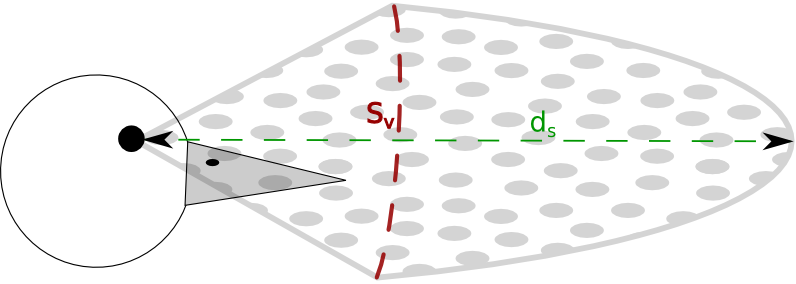
\includegraphics[scale=0.45]{./images/verticalFow.png}
		\label{fig:vFOV}
		\caption{Birds vertical field of view.}
\end{figure}	
	
	
\begin{figure}[b]
\centering
	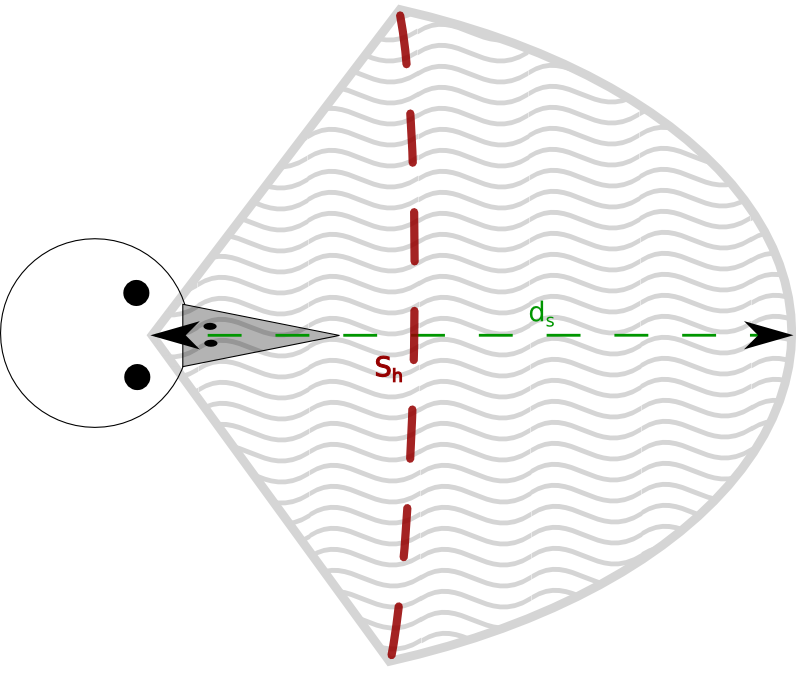
\includegraphics[scale=0.375]{./images/hFow.png}
	\label{fig:hFOV}
	\caption{Birds horizontal field of view.}
\end{figure}	
	




\subsection{Flight Model}
Bird $b$ flight at step $i$ is described by its $3$-dimensional space vectors
position $\vec{p}_b^i=\expval{p^i_x,p^i_y,p^i_z}$ and velocity
$\vec{v}_b^i=\expval{v^i_x,v^i_y,v^i_z}$, that correspond to its current sight
direction. 


The evolution of the bird's  velocity over time is regulated by
the following:

\begin{align}
\label{eq:birdCumulativeVelocities}
\vec{v}_b^{i+1} = (r \sin \theta' \cos \phi',r \sin \theta' \sin \phi',r
\cos\theta')
\end{align}




where:
\begin{itemize}
  \item $
     \theta' = \begin{cases}
    \theta_d &\mbox{ if }  |\theta_b - \theta_d| < \theta_{max}\\
    \theta_b + \theta_{max} &\mbox{ otherwise }\\
    \end{cases}
  $ \hfill \\
  
    \item $
     \phi' = \begin{cases}
    \phi_d &\mbox{ if }  |\phi_b - \phi_d| < \phi_{max}\\
    \phi_b + \phi_{max} &\mbox{ otherwise va aggiustato il segno a seconda se
    bisogna andare a destra o sinistra}\\
    \end{cases}
  $ \hfill \\ 
   

\item $ \vec{v}_d^i = \mu_c \vec{v}_c + \mu_s\vec{v}_s + \mu_a \vec{v}_a + \mu_{a} \left(
\vec{{\tau}_i} + \vec{\Gamma}_i \right) + \vec{\omega}_i $

\begin{itemize}
	\item $\mu_c$, $\mu_s$, $\mu_a$ are the cohesion, separation and alignment coefficient (social coefficients) and $\mu_a$ is the avoidance coefficient. 
\end{itemize}
\item  $\vec{v}^i_c$,$\vec{v}^i_s$, $\vec{v}^i_a$ are the  \textit{social velocities} \cite{Hemelrijk}
  \begin{itemize}
    \item $\vec{v}^i_c$, the cohesion velocity that has direction parallel to the
    line that pass through $\vec{p}_b^i$ and the average position of its neighbors
    \item $\vec{v}^i_s$, the separation velocity, keep the bird at a minimum
    safety distance from its flockmates
    \item  $\vec{v}^i_c$, the align velocity, synchronize boids heading
  \end{itemize}
 \item $\theta_d,\theta_b$ are the polar angle of the velocity vector
 $\vec{v}^i_b$ and $\vec{v}^i_d$ respetively
 \item $\phi_d,\phi_b$ are the azimuthal angle of the velocity vector
 $\vec{v}^i_b$ and $\vec{v}^i_d$ respetively


\end{itemize}


\subsection{Bird's Field of View}
Each bird has a limited visual capacity described by its field of view (FOV).
This implies that it can only perceive objects that are within its FOV. Bird
$o$'s FOV $\mathcal{F}_p$, is here defined as the set of points $p_n$ that
satisfy equations \ref{eq:fov1},\ref{eq:fov2} and \ref{eq:fov3}. In order an
object  $n$ to be within the  observer $o$'s neighborhood, it must fall within
its viewing frustum i.e. the polar and azimuthal angle between observer's view
direction and the object are less or equal than $s_h$ and $s_v$ respectively
and the distance between them should be less than the maximum sight distance of the
observer $s_d$.
Let $\vb{p'_n}=\expval{p^x_n-v^x_o,p^y_n-v^y_o,p^z_n-v^z_o}$ the position vector of the object $n$ in the $o$'s frame of reference then $n$ is $o$'s neighbor if and only if the followings hold:
\begin{equation}
\label{eq:fov1}
	\delta_s = || \vb{p_o} - \vb{p_n} ||,\; \delta_s \leq d_s 
\end{equation}
 
\begin{equation}
\label{eq:fov2}
	\frac{-s_h}{2} \leq \theta \leq \frac{+s_h}{2}
\end{equation}

\begin{equation}
\label{eq:fov3}
\frac{-s_v}{2} \leq \phi \leq \frac{+s_v}{2}
\end{equation}
where: 
\begin{align*}
 &\phi = \arccos
	\left(\frac{p'^z_n}{\sqrt{(p'^x_n)^2 + (p'^y_n)^2 + (p'^z_n)^2}}\right) \\
	&\theta = atan2 \left(\frac{p'^y_n}{p'^x_n} \right) 
\end{align*}
See appendix \ref{app:cartToSpherical} for precide definition of $atan2$
and further details.
	
	
% 	\begin{align}
% 		\label{eq:fov1}
% 		&\delta_p = |\vec{p}_{n} - \vec{p}_{o}|,\;\; \delta_p \leq d_s \\
% 		&\Delta_\alpha = \left|\frac{\alpha - \alpha'}{2}\right|,\;\; 0 \leq
% 		\Delta_\alpha \leq s_h\label{eq:fov2} \\
% 		&\Delta_\beta = \left|\frac{\beta - \beta'}{2}\right|,\;\; 0 \leq \Delta_\beta
% 		\leq s_v \label{eq:fov3}
% 	\end{align}
% where
% $\vb{p_r}=\expval{x',y',z'} = \vec{p}_{n} - \vec{p}_{o}$,
% $\vb{p_o}=\expval{x,y,z}$,
% $\alpha = arctan \left[\frac{y}{x}\right]$,
% $\beta =arctan \left[\frac{z}{\sqrt{x^2 + y^2}}\right]$,
% $\alpha' = arctan\left[\frac{y'}{x'}\right]$,
% $\beta' = arctan \left[\frac{z'}{\sqrt{x'^2 + y'^2}}\right]$.



\subsection{Cohesion}
Cohesion is a flight behavior that attracts a bird to centroid of  its perceived
neighborhood. 
In formal terms \(\vec{C}_b^i\), the bird b's centroid at time $i$, is given by:

\begin{align}
 \vec{C}_b^i = \frac{1}{|\mathcal{N}_b|}\sum_{n=1}^{|\mathcal{N}_b|}{\vec{p}_n  \frac{d_{i,j}}{d_s}}
\end{align}

where:

\begin{enumerate}
\item \(\mathcal{N}_b\) the set of birds in b's FOV.
\item \(\vec{p}_n\) is the position of $n \in \mathcal{N}_b$
\item \(d_{i,j}\) is the distance between bird \emph{b} and its neighbor
	\emph{c}

\end{enumerate}

The $b$'s cohesion vector \(\vec{v}_c\) is then defined as follows.

\begin{equation}
\vec{v}_c^i =
	\begin{cases}
	 \frac{\vec{C}_b^i - \vec{p}_b}{|| \vec{C}_b^i - \vec{p}_b ||} +
		a, &\mbox{ if } 0 < |\vec{v}_d| \leq v_p \\
		v_p, &\mbox{ otherwise } 
	\end{cases}
\end{equation}

\subsection{Separation}
\label{sect:separation}
A bird try to keep certain distance between itself and
its neighbors. Bird $b$'s separation velocity $\vec{S}_b^i$ at time $i$ is given
by:


\begin{equation}
\vec{S}_b^i = 
	\begin{cases}
	 \left[\sum_{j \in \mathcal{N}_b}{\frac{\vec{p}_b -
\vec{p}_j}{||\vec{p}_b - \vec{p}_j||}} \;f_s\right] + a ,&\mbox{if } 0 < |\vec{S}_i|
\leq v_p\\
		v_p, &\mbox{ otherwise } 
	\end{cases}
\end{equation}



where:

\begin{enumerate}
\item \(\mathcal{N}_b\) is the number of neighbors
\item $
	f_s = \begin{cases}
	0 &\mbox{ if }  d_{i,j} > d_{min}\\
	1 - \frac{d_{i,j}}{d_{min}} &\mbox{ otherwise}
	\end{cases}$
\end{enumerate}

\subsection{Alignment}
A bird tries to match its velocity (speed and heading) with those of
nearby flockmates, a behavior called velocity alignment. Real life birds only consider a relatively small number flockmates while performing this behavior and it usually is about seven neighbors\cite{Hemelrijk}.
In formal terms, bird $b$'s alignment \(\vec{A}_b^i\) is here defined as (equation \ref{eq:alignment})

\begin{align}
  \vec{A}_i = \left[\sum_{j \in \mathcal{N}'_b}{\vec{v_j}}\;f_a\right] + a, \;\;0 < |\vec{A}_i| \leq v_p
  \label{eq:alignment}
\end{align}

where:

\begin{enumerate}
\item \(\mathcal{N}'_b \subseteq \mathcal{N}_b\) is the set of birds considered by $b$ for the alignment (e.g. the nearests).
\item \(\vec{v}_j\) is the $j$'s velocity.
\item \(f_a\) is the alignment coefficient. Let \(d_{i,j}\) the distance between bird \emph{i} and \emph{j} then \(f_a\) is given by:

\begin{equation*}
	f_a = \begin{cases}
	0 &\text{, if $ d_{i,j} > d_a$}\\
	1- \frac{d_{i,j}}{d_a} &\text{, otherwise}
	\end{cases}
\end{equation*}
\end{enumerate}

\subsection{Other species and predator avoidance}
\textsc{ACIADDRI} is a multi-agent with multiple group model where each group correspond to a different bird's specie or to the group of predators. 
Different species interaction is described in section \ref{sect:otherSpecieAvoidance} and predator avoidance in section \ref{sect:predatorAvoidance}.
\begin{enumerate}[-]
	\item \textbf{Other species avoidance}
	\label{sect:otherSpecieAvoidance}
	This behavior is similar to \textit{separation} (see section \ref{sect:separation}) with the difference that a only birds from other species are taken into consideration. In formal terms the other specie avoidance vector  \(\vec{\tau}_i\) is given by:
	
	\begin{equation}
	\vec{\tau}_i = 
		 \left[\sum_{j \in \mathcal{N}_b}{\frac{\vec{p}_b -\vec{p}_j}{||\vec{p}_b - \vec{p}_j||}} \;f_s\right] + a 
	\end{equation}
	where:
	
	\begin{enumerate}
	\item \(\mathcal{N}_b\) is the number of neighbors of specid different from the one of $b$
	\item $
		f_s = \begin{cases}
		0 &\mbox{ if }  d_{i,j} > r_s\\
		1 - \frac{d_{i,j}}{r_s} &\mbox{ otherwise}
		\end{cases}$
	\end{enumerate}
	
	
	\item \textbf{Predator avoidance}
	\label{sect:predatorAvoidance}
	The predator avoidance vector is computed by taking in consideration position and velocity (speed and heading) of all the  predators within the bird's FOV. Intuitively birds will flee from the future (step $i+1$) centroid of predators's position. Formally the predator avoidance vector $\vec{\Gamma}_b^i$ is defined as follows:
	
	\begin{align}
	\vec{\Gamma}_b^i = \left[\sum_{j \in \mathcal{P}_b }^m{\frac{\vec{p}_i -
	(\vec{p}_j+\vec{v}_j)}{||\vec{p}_i - (\vec{p}_j+\vec{v}_j)||}} \;f_{p}\right] +
	a, \;\;0 < |\vec{\Gamma}_i| \leq v_p
	\end{align}
	
	where:
	
	\begin{enumerate}
	\item \(\mathcal{P}_b\) is the $b$'s set of predators
	\item $	f_{p} = \begin{cases}
		0 &\mbox{ if }  d_{i,j} > r_p\\
		1 - \frac{d_{i,j}}{r_p} & \mbox{ otherwise}
		\end{cases}
	$ \hfill \\
	 is the predator avoidance coefficient.
	\end{enumerate}
\end{enumerate}

\subsection{Wandering}
When the neighborhood  of a bird is empty it flies pseudo-randomly in the space. This kind of behavior is called \textit{wandering}. 
Wandering is obtained combining a current and a random direction 
\begin{equation*}
    \vec{\omega}_b^i =  
		\begin{cases} 
			0 &\mbox{if } \mathbb{N} \neq \emptyset \\ 
			\frac{\vec{s}}{|\vec{s}|}\;w_r+w_d,\; 0 < |\vec{\omega}_i| \leq v_p & \mbox{otherwise }. 
		\end{cases}
\end{equation*}
